%!TEX root = ../template.tex
%%%%%%%%%%%%%%%%%%%%%%%%%%%%%%%%%%%%%%%%%%%%%%%%%%%%%%%%%%%%%%%%%%%%
%% abstrac-en.tex
%% NOVA thesis document file
%%
%% Abstract in English([^%]*)
%%%%%%%%%%%%%%%%%%%%%%%%%%%%%%%%%%%%%%%%%%%%%%%%%%%%%%%%%%%%%%%%%%%%

\typeout{NT FILE abstrac-en.tex}

% Compared to strain gages and extensometers, the amount of information gathered about the fine details of deformation during mechanical tests is increased due to the ability to provide both local and average data using digital image correlation.


%The tracking creates in-plane displacement patterns, from which strains are calculated. Multiple cameras triangulating on the points can map out-of-plane displacements as well. During the test, the movement of the spots are recorded digitally, and appropriate derivatives of displacement are taken to arrive at strains.



Digital image correlation, DIC, is an optical full-field strain measurement technique for 2D or 3D ANALYSIS. In a simpler manner of speech, DIC consists in the comparison of two or more images of an object before and after its deformation.\\
This technique has first been applied to digital images in 1975 and, thanks to the progress of technology and improvement of cameras, it has become a reliable technique for many present-day applications like, image analysis, velocimetry, and strain estimation.\\

In order to perform the technique, the sample surface is painted with a solid base colour, typically black or white, and then sprayed with a contrasting colour, creating distinct patterns all over it. Those patterns are then taken as a reference in the control picture and compared, in terms of displacement and deformation, with the ones on the following deformed pictures, from which the strains can also be calculated through.\\

This method of analysis is possible by turning the pictures into matrices, where each of its units represent subsets or blocks of pixels, correlating the position of such pixels in the original and deformed PICTURES/MATRICES, as shown in the figure~\ref{fig:dic}, thence the need of creating distinct patterns.\\

\begin{figure}[h!]
	\centering
	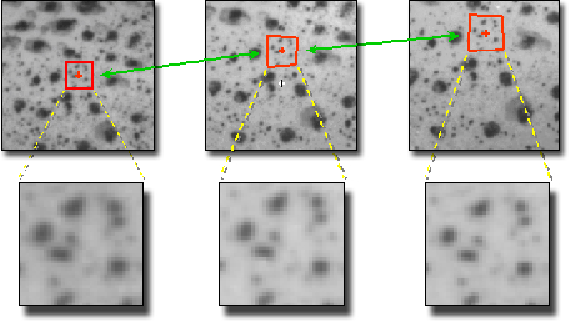
\includegraphics[scale=1]{DIC}
	\caption{Example of image correlation}
	\label{fig:dic}
\end{figure}

The developed software, on which this paper is focused on, is a 3D DIC software, whose code was written in python, and which is meant to be open-source. The software was BASED and tested with the aid of Manta GigE Allied Vision digital cameras. %EACH POSITIONED IN XXXX ANGLES AND CAPABLE OF MICRO ANALYSIS???' REFAZER FRASE
Having the codebase finished, the next step consisted on making it accessible for its users through a \textbf{G}raphical \textbf{U}ser \textbf{I}nterface, GUI.

Throughout the course of this paper, it will be SHOWED/EXPLAINED the progress/PROCESS and deliberations taken in order to build the GUI. The objective was to have a LIGHT-LOOKING GUI, where the user would be capable of using it in an objective and intuitive way.

%It is also possible to estimate shifts to a finer resolution than the resolution of the original images, which is often called "subpixel" registration because the measured shift is smaller than an integer pixel unit. 






% https://www.sciencedirect.com/topics/engineering/digital-image-correlation
% Donald F. Adams, Thomas J. Whitney, in Comprehensive Composite Materials II, 2018
% M.A. Rastak, Mahmood M. Shokrieh, L.Barrallier, R. Kubler, S.D. Salehi, in Residual Stresses in Composite Materials (Second Edition), 2021
% W. Broughton, in Adhesives in Marine Engineering, 2012
% https://en.wikipedia.org/wiki/Digital_image_correlation_and_tracking


